\chapter{Testen der Algorithmen} \label{Kap5}

Im letzten Schritt werden die Kartierungsalgorithmen getestet. Dazu werden verschiedene Szenarien dargestellt. Für jedes Szenario werden Karten durch das Ausführen der Kartierungsalgorithmen erstellt.

Im ersten Szenario wurde aus Tischen ein Rechteck aufgebaut. Ein Tisch ist 1,75m lang. Demnach ist die Breite des Aufbaus 1,75m und die Länge 3,90m, da es auf beiden Seiten noch einen Offset von 20cm gibt. Der Pioneer soll in verschiedenen Arten dort außen herum fahren.

\begin{figure}[t]
  \centering
  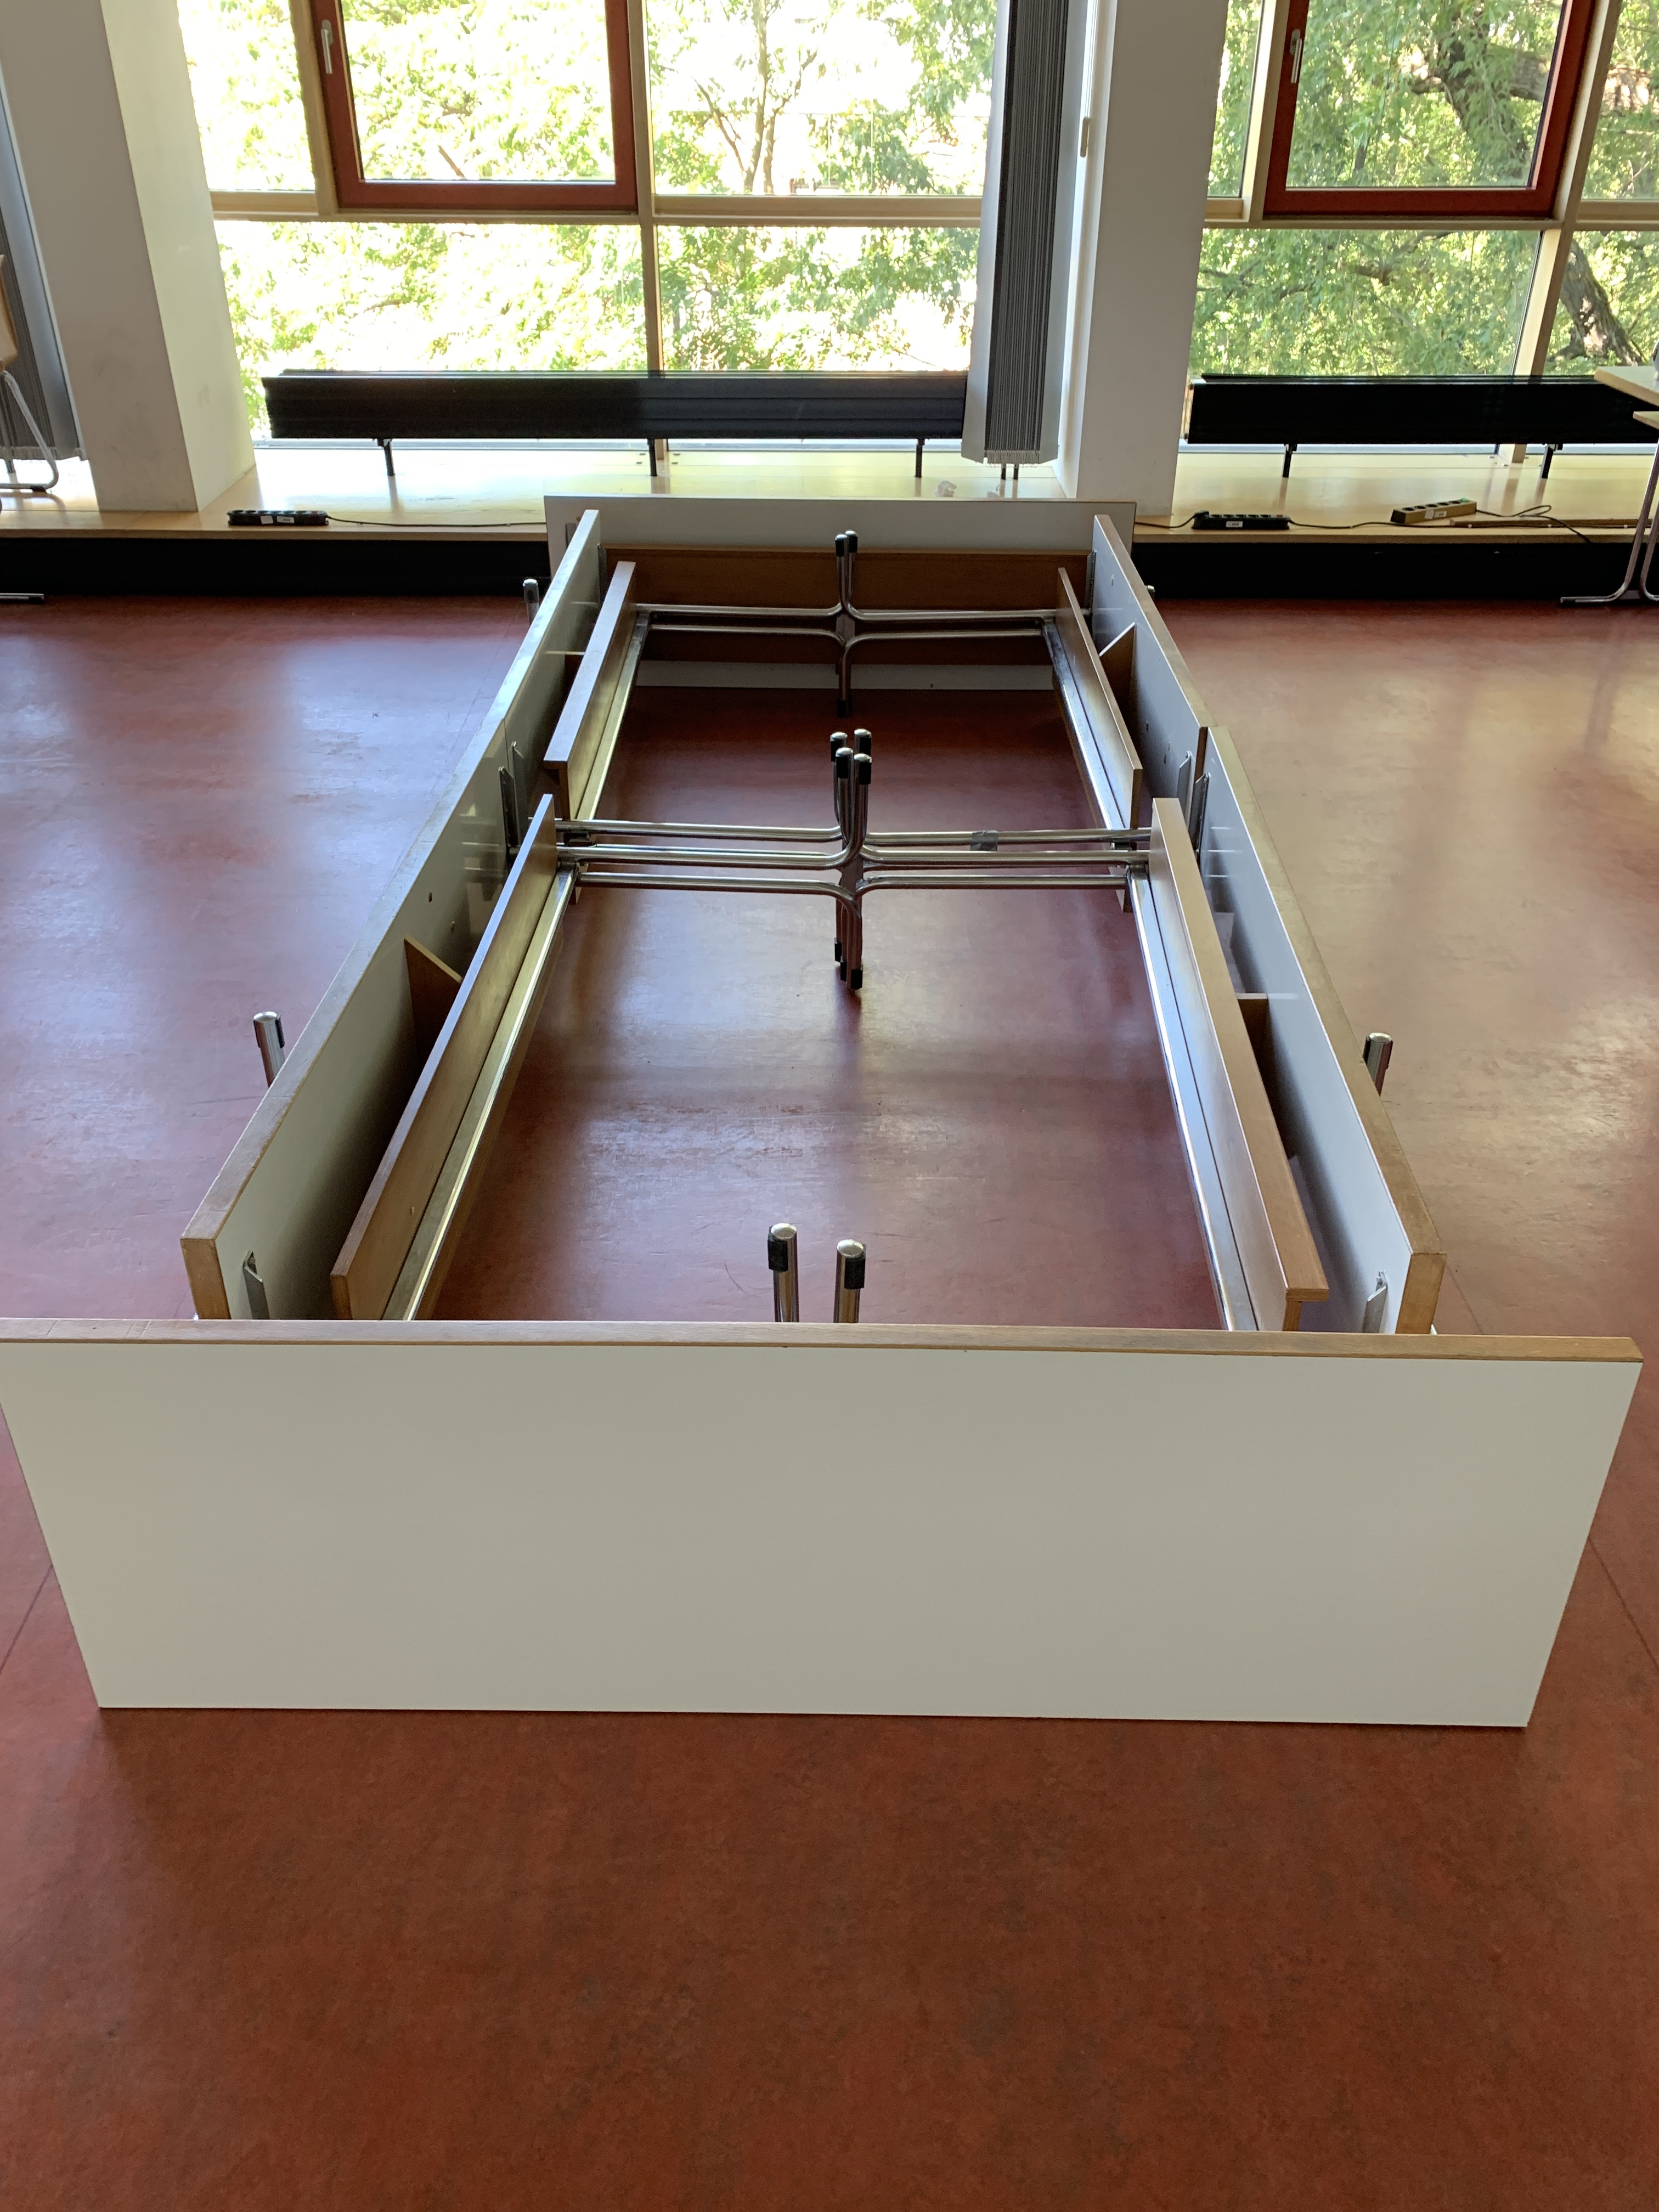
\includegraphics[height=8cm]{kapitel5/testszenario_1}
  \caption{Szenario-Aufbau: Um ein Rechteck fahren}
  \label{Kap5:Szenario1}
\end{figure}

Die erste Aufgabe besteht darin, um das aufgestellte Rechteck zu fahren. Dabei wird möglichst gerade und in einer durchschnittlichen Geschwindigkeit gefahren. Die nächste Aufgabe baut auf der ersten Aufgabe auf. Der Unterschied ist, dass diesmal versucht wird, so schnell wie der Pioneer fahren kann, zu fahren. Die dritte Aufgabe baut ebenfalls auf der ersten Aufgabe auf. Diesmal darf nur rückwärts gefahren werden. In der vierten Aufgabe darf nur in Schlangenlinien gefahren werden.

Im zweiten Szenario soll der Pioneer durch die Vordertür einen Raum betreten und diesen durch die Hintertür wieder verlassen. Das Ziel ist es, auf einer größeren Fläche den Kreis von Scans wieder zu schließen. Die Aufgabe besteht darin, in einer durchschnittlichen Geschwindigkeit durchzufahren und wieder am Endpunkt anzukommen.

Für die Durchführung wird für jede Aufnahme ein Bag-File aufgenommen. Dieses wird beim Auswerten für jeden Algorithmus abgespielt. Dafür dienen die Offline-Launch-Files, welche in \autoref{Kap4} definiert sind.

\section{cartographer}

\begin{figure}[b]
  \centering
  \begin{subfigure}[b]{0.4\linewidth}
    \centering
    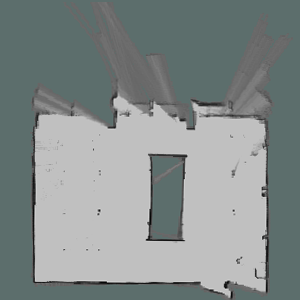
\includegraphics[scale=0.8]{kapitel5/cartographer_umdentisch}
    \subcaption{Normal}\label{kap5:cartographer1}
  \end{subfigure}%
  \qquad
  \begin{subfigure}[b]{.4\linewidth}
    \centering
    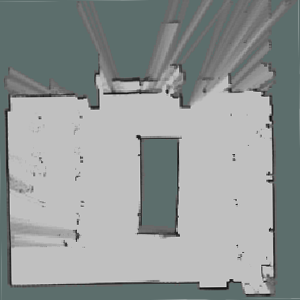
\includegraphics[scale=0.8]{kapitel5/cartographer_umdentischrueckwaerts}
    \subcaption{Rückwärts}\label{kap5:cartographer2}
  \end{subfigure}\\
  \vspace{2\floatsep}
  \begin{subfigure}[b]{.4\linewidth}
    \centering
    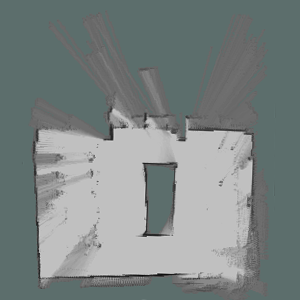
\includegraphics[scale=0.8]{kapitel5/cartographer_umdentischschnell}
    \subcaption{Schnell}\label{kap5:cartographer3}
  \end{subfigure}%
    \qquad
  \begin{subfigure}[b]{.4\linewidth}
    \centering
    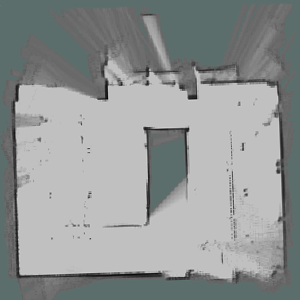
\includegraphics[scale=0.8]{kapitel5/cartographer_umdentischzickzack}
    \subcaption{Schlangenlinien}\label{kap5:cartographer4}
  \end{subfigure}%
  \qquad
  \caption{cartographer: Resultat der Aufnahmen des ersten Szenarios}
  \label{kap5cartographerResultateSzenario1}
\end{figure}

Der Cartographer konnte die Karten zunächst nur ziemlich ungenau zeichnen, da es Probleme mit der Positions- und Drehungsbestimmung des Roboters gab. Der Algorithmus hat diesen Wert falsch geschätzt.

Durch das Aktivieren des \textit{use\_online\_correlative\_scan\_matching} und dem Setzen von \textit{TRAJECTORY\_BUILDER\_2D.ceres\_scan\_matcher.translation\_weight} auf 10
 sowie \textit{TRAJECTORY\_BUILDER\_2D.ceres\_scan\_matcher.rotation\_weight} auf 2 konnten gute Ergebnisse erzielt werden.
 
Das Resultat des ersten Szenarios findet man in \autoref{kap5cartographerResultateSzenario1}. Die Teilabbildung \autoref{kap5:cartographer1} zeigt die normale Auswertung, bei der das Rechteck ziemlich genau dargestellt wird. Auch die Aufgabe in \autoref{kap5:cartographer2}, rückwärts um das Rechteck zu fahren, wird sehr präzise dargestellt. Bei der schnellen Fahrt in \autoref{kap5:cartographer3} ist das Rechteck zu erkennen. Dieses ist allerdings nicht exakt gerade gezeichnet. Gründe dafür könnten sein, dass der Algorithmus zu wenige Daten erhalten hat oder durch die schnellen Bewegungen Ungenauigkeiten in der Odometrie entstanden sind. In \autoref{kap5:cartographer4} wurden Schlangenlinien um das Rechteck gefahren. Dennoch ist das Rechteck gut zu erkennen. Lediglich hat im unteren Teil ein Scan das Rechteck geschnitten. Da dort die Aufnahme geendet hat, hatte der Cartographer keine Zeit mehr, dieses durch weitere Scans zu optimieren. Insgesamt haben alle Auswertungen bis auf die Auswertung \autoref{kap5:cartographer3}, bei der schnell gefahren wurde, den gesamten Umriss des Raums gut erkannt.

\begin{figure}[b]
  \centering
  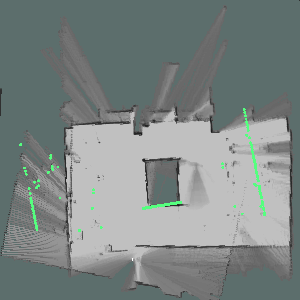
\includegraphics[height=8cm]{kapitel5/cartographer_umdentischmitimu}
  \caption{cartographer: Resultat der Aufnahmen des ersten Szenarios mit IMU}
  \label{kap5cartographerResultateSzenario1a}
\end{figure}

In \autoref{kap5cartographerResultateSzenario1a} wurde eine \ac{IMU} verwendet, um die Auswertung zu verbessern. Dabei gab es Probleme mit der Kalibrierung und der Integration in das eigene \ac{ROS}-Modul, so dass die Auswertung dadurch eher ungenauer wurde. Die \ac{IMU} wurde durch die Konfiguration \textit{TRAJECTORY\_BUILDER\_2D.use\_imu\_data} aktiviert.

Im zweiten Szenario in \autoref{kap5cartographerResultateSzenario2} konnte der Cartographer ohne \ac{IMU} die Scans wieder zusammenfinden und eine ziemlich genaue Karte erstellen.

\begin{figure}[b]
  \centering
  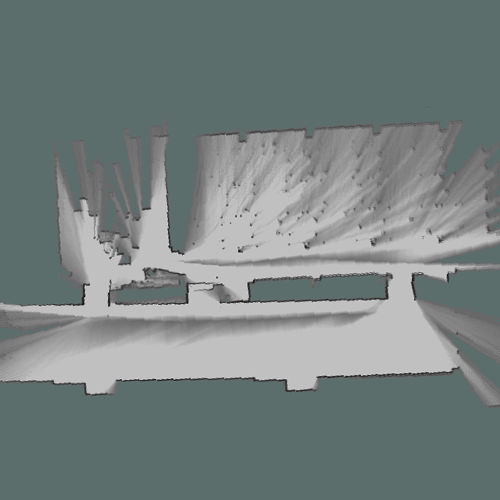
\includegraphics[height=6cm]{kapitel5/cartographer_a207}
  \caption{cartographer: Resultat der Aufnahmen des zweiten Szenarios}
  \label{kap5cartographerResultateSzenario2}
\end{figure}

\section{gmapping}

\begin{figure}[b]
  \centering
  \begin{subfigure}[b]{0.4\linewidth}
    \centering
    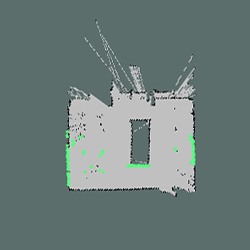
\includegraphics[scale=0.8]{kapitel5/gmapping_umdentisch}
    \subcaption{Normal}\label{kap5:gmapping1}
  \end{subfigure}%
  \qquad
  \begin{subfigure}[b]{.4\linewidth}
    \centering
    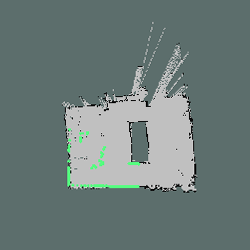
\includegraphics[scale=0.8]{kapitel5/gmapping_umdentischrueckwaerts}
    \subcaption{Rückwärts}\label{kap5:gmapping2}
  \end{subfigure}\\
  \vspace{2\floatsep}
  \begin{subfigure}[b]{.4\linewidth}
    \centering
    
\includegraphics[scale=0.8]{kapitel5/gmapping_umdentischschnell}
    \subcaption{Schnell}\label{kap5:gmapping3}
  \end{subfigure}%
    \qquad
  \begin{subfigure}[b]{.4\linewidth}
    \centering
    
\includegraphics[scale=0.8]{kapitel5/gmapping_umdentischzickzack}
    \subcaption{Schlangenlinien}\label{kap5:gmapping4}
  \end{subfigure}%
  \qquad
  \caption{gmapping: Resultat der Aufnahmen des ersten Szenarios}
  \label{kap5GmappingResultateSzenario1}
\end{figure}

Bei gmapping waren keine Anpassungen nötig, um vernünftige Karten erstellen zu können. In \autoref{kap5GmappingResultateSzenario1} werden die Ergebnisse präsentiert. Die Auswertung \autoref{kap5:gmapping1} ist gut gelungen, da das Rechteck gut erkennbar ist. Beim Rückwärtsfahren in Auswertung \autoref{kap5:gmapping2} ist sowohl der Raum als auch das Rechteck ungenau gezeichnet. Beim Schnellfahren in \autoref{kap5:gmapping3} ist das Rechteck wieder präzise gezeichnet. Es fehlen dort lediglich einige Messwerte, um den Raum auszufüllen. Auch beim Fahren in Schlangenlinien in \autoref{kap5:gmapping4} ist gmapping stabil und produziert ein präzises Resultat. Das gmapping hat außer beim Rückwärtsfahren immer präzise funktioniert.

Auch beim zweiten Szenario in \autoref{kap5GmappingResultateSzenario2} produziert der Algorithmus ein gutes Ergebnis, da die Scans nach dem Zurückkehren guten zusammengefunden wurden.

\begin{figure}[b]
  \centering
  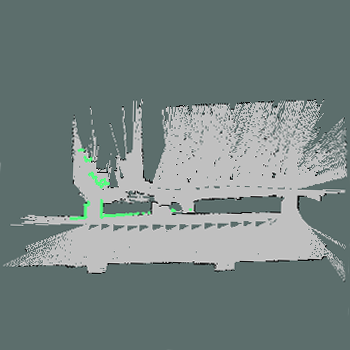
\includegraphics[height=8cm]{kapitel5/gmapping_a207}
  \caption{gmapping: Resultat der Aufnahmen des zweiten Szenarios}
  \label{kap5GmappingResultateSzenario2}
\end{figure}

\section{hector\_mapping}

\begin{figure}[b]
  \centering
  \begin{subfigure}[b]{0.4\linewidth}
    \centering
    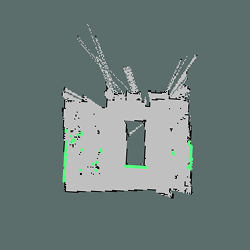
\includegraphics[scale=0.8]{kapitel5/hector_mapping_umdentisch}
    \subcaption{Normal}\label{kap5:hector_mapping1}
  \end{subfigure}%
  \qquad
  \begin{subfigure}[b]{.4\linewidth}
    \centering
    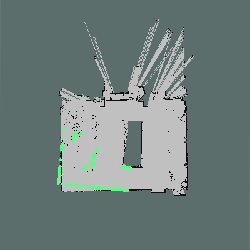
\includegraphics[scale=0.8]{kapitel5/hector_mapping_umdentischrueckwaerts}
    \subcaption{Rückwärts}\label{kap5:hector_mapping2}
  \end{subfigure}\\
  \vspace{2\floatsep}
  \begin{subfigure}[b]{.4\linewidth}
    \centering
    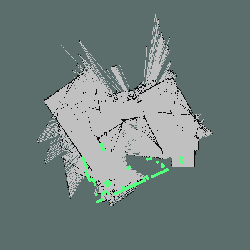
\includegraphics[scale=0.8]{kapitel5/hector_mapping_umdentischschnell}
    \subcaption{Schnell}\label{kap5:hector_mapping3}
  \end{subfigure}%
    \qquad
  \begin{subfigure}[b]{.4\linewidth}
    \centering
    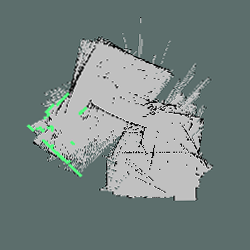
\includegraphics[scale=0.8]{kapitel5/hector_mapping_umdentischzickzack}
    \subcaption{Schlangenlinien}\label{kap5:hector_mapping4}
  \end{subfigure}%
  \qquad
  \caption{hector\_mapping: Resultat der Aufnahmen des ersten Szenarios}
  \label{kap5HectorMappingResultateSzenario1}
\end{figure}

Auch beim hector\_mapping waren keine Anpassungen nötig, um vernünftige Karten erstellen zu können. Die Karte in \autoref{kap5:hector_mapping1} hat wie in den vorherigen Algorithmen ebenfalls gute Ergebnisse erzielt. Beim Rückwärtsfahren in Karte \autoref{kap5:hector_mapping2} ist der linke Teil des Rechtecks verrutscht. Ansonsten ist diese Karte gut gelungen. Kaum gut gelungen sind die Karten, die durch Schnellfahren oder durch Schlangenlinien in \autoref{kap5:hector_mapping3} und \autoref{kap5:hector_mapping4} erzeugt wurden. Bei diesen ist gar kein Rechteck erkennbar und diese sind ziemlich verrutscht. Das hector\_mapping hat hier also nur gut funktioniert, wenn vorwärts oder rückwärts in einer normalen Geschwindigkeit gefahren wurde. Zu viele oder zu schnelle Kurven haben dagegen nicht funktioniert.

Auch im zweiten Szenario in \autoref{kap5HectorMappingResultateSzenario2} haben zu viele Kurven das Ergebnis ungenau gemacht. Der Rest der Karte ist ansonsten präzise.

\begin{figure}[b]
  \centering
  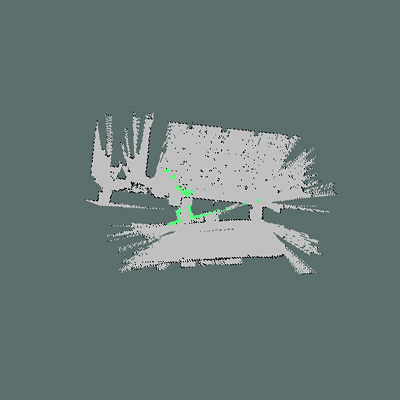
\includegraphics[height=8cm]{kapitel5/hector_mapping_a207}
  \caption{hector\_mapping: Resultat der Aufnahmen des zweiten Szenarios}
  \label{kap5HectorMappingResultateSzenario2}
\end{figure}

\section{Vergleich}

\autoref{tab:vglkartierungsalgorithmen} stellt dar, wie die einzelnen Kartierungsalgorithmen nach einigen Kriterien abgeschlossen haben. 

Zunächst einmal sind die Konfigurationsmöglichkeiten der Algorithmen von Bedeutung. Da bietet der Cartographer eine große Auswahl mit einer guten Dokumentation. Die anderen Algorithmen lassen sich auch konfigurieren, allerdings ist mit dem Cartographer einfach viel mehr möglich, wie zum Beispiel die 3D-Kartierung oder das Verwenden einer \ac{IMU}.

Alle Algorithmen konnten den ersten Test problemlos durchführen. Probleme hingegen gab es beim Rückwärts, Schnell oder Schlangenlinien fahren. Insgesamt schnitt der Cartographer am besten ab, da dieser alle Tests nach einigen Optimierungen der Konfiguration bestanden hat. Der gmapping-Algorithmus hatte Probleme beim Rückwärtsfahren und der hector\_mapping-Algorithmus konnte die Kartierung für eine schnelle Fahrt und eine Fahrt in Schlangenlinien nicht gut durchführen.

Der Test für die \ac{IMU} schlug zwar auf dem Cartographer auf Grund von einer falschen Kalibrierung und einem fehlerhaften \ac{ROS}-Package fehl, dennoch ist es positiv, dass der Algorithmus diese Option als einziger anbietet.

\begin{table}[b]
  \caption{Vergleich der Kartierungsalgorithmen}
  \label{tab:vglkartierungsalgorithmen}
  \centering
  \begin{tabular}{lccc}
    \toprule
    & Cartographer & gmapping & hector\_mapping\\
    \midrule
    Konfigurationsmöglichkeiten	& \harveyBallFull & \harveyBallHalf & \harveyBallHalf \\
    Normal fahren	& \harveyBallFull & \harveyBallFull & \harveyBallFull \\
    Rückwärts fahren	& \harveyBallFull & \harveyBallThreeQuarter & \harveyBallFull\\
    Schnell fahren	& \harveyBallFull & \harveyBallFull & \harveyBallQuarter\\
    Schlangenlinien fahren & \harveyBallFull & \harveyBallFull & \harveyBallQuarter\\
    IMU & \harveyBallQuarter & - & -\\
    \bottomrule
  \end{tabular}
\end{table}